\chapter{Models}
Our algorithm will generate an emulation using vertex disjoint subgraph homeomorphism. For this purpose, we will use vertex-multilabeled directed simple graphs as defined in Definition \ref{def:graph}. In these graphs we will:

\begin{itemize}
\item ..model a wire as a vertex that may be connected with any number of vertices in either direction of types ``$arc$", any number of incoming edges from ``$port\_out$" vertices and any number of outgoing edges to ``$port\_in$" edges.
\item ..model a transistor as a vertex with a label ``$arc$" and a label ``$configurable$" for configurable transistors or label ``$unconfigurable$" for unconfigurable transistors (that are not counted towards label compatibility). It has an incoming edge from the source ``$wire$" of the transistor and an outgoing edge to the target ``$wire$" of the transistor.
\item ..model a LUT as a vertex with label $``lut"$ that only has connections from vertices with label ``$port\_in$" and to vertices with label ``$port\_out$".
\item ..model a register as a vertex with label ``$register$" that only has connections from vertices with label ``$port\_in$" and to vertices with label ``$port\_out$"..
\item ..model an input of a component as a vertex with label ``$port\_in$" and an outgoing directed edge towards a ``$lut$" or ``$register$" vertex and an incoming edge from a ``$wire$" vertex.
\item ..model an output of a component as a vertex with label ``$port\_out$" and an incoming directed edge from a ``$lut$" or ``$register$" vertex and an outgoing edge to a ``$wire$" vertex.
\end{itemize}

An example of such am model is shown in Figure \ref{fig:graphmodel-logiccell} where a graph model is shown of the logic cell in Figure \ref{fig:logiccell}.

\begin{figure}
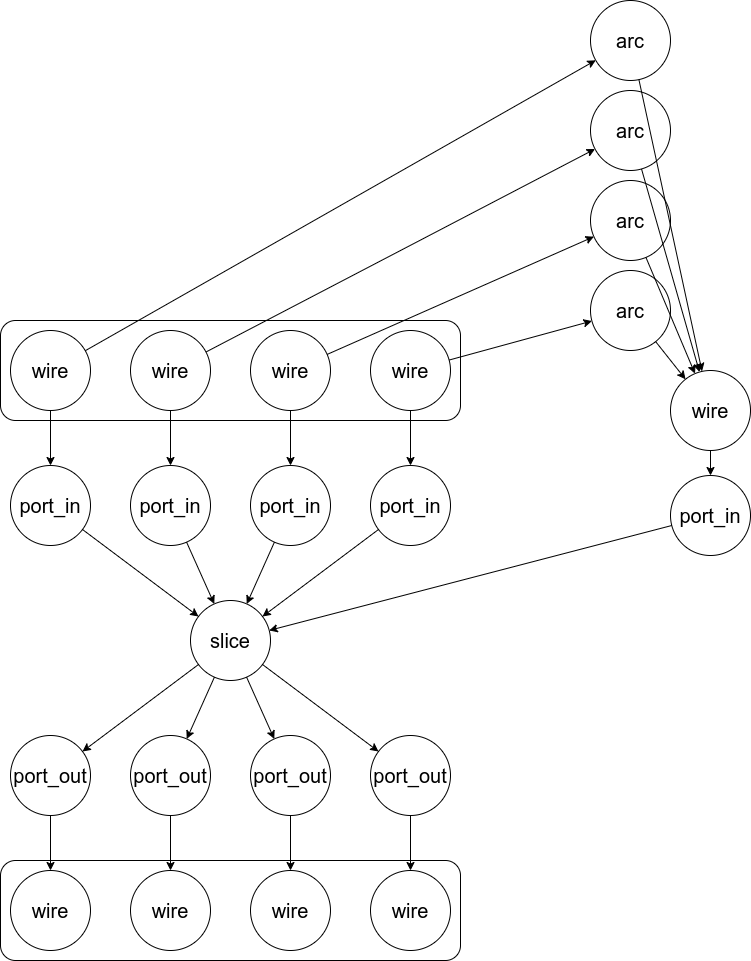
\includegraphics[width=\textwidth]{images/modelOfCell.png}
\caption{Graph model of the logic cell shown in Figure \ref{fig:logiccell}}
\label{fig:graphmodel-logiccell}
\end{figure}
